\documentclass{standalone}
\usepackage{tikz}
\usetikzlibrary{patterns, positioning}

\begin{document}
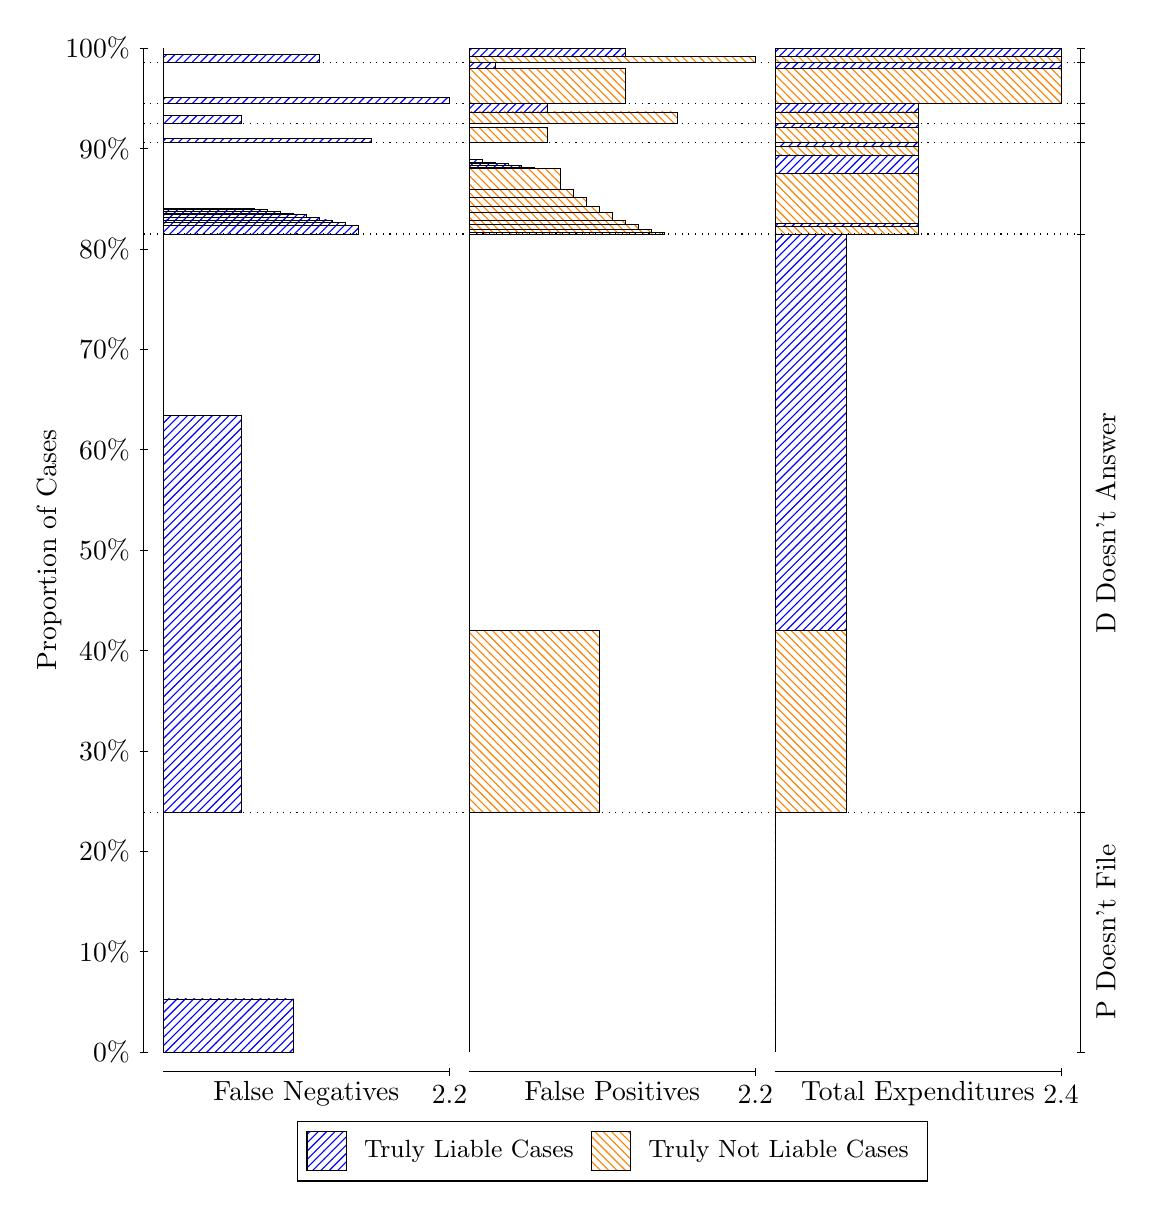
\begin{tikzpicture}
\draw[black, very thin] (1.5,1.75) -- (1.5,14.5);
\node[rotate=90, anchor=center] at (0.3, 8.125) {Proportion of Cases};
\draw[black, very thin] (1.45,1.75) -- (1.55,1.75);
\node[anchor=east] at (1.45, 1.75) {0\%};
\draw[black, very thin] (1.45,3.025) -- (1.55,3.025);
\node[anchor=east] at (1.45, 3.025) {10\%};
\draw[black, very thin] (1.45,4.3) -- (1.55,4.3);
\node[anchor=east] at (1.45, 4.3) {20\%};
\draw[black, very thin] (1.45,5.575) -- (1.55,5.575);
\node[anchor=east] at (1.45, 5.575) {30\%};
\draw[black, very thin] (1.45,6.85) -- (1.55,6.85);
\node[anchor=east] at (1.45, 6.85) {40\%};
\draw[black, very thin] (1.45,8.125) -- (1.55,8.125);
\node[anchor=east] at (1.45, 8.125) {50\%};
\draw[black, very thin] (1.45,9.4) -- (1.55,9.4);
\node[anchor=east] at (1.45, 9.4) {60\%};
\draw[black, very thin] (1.45,10.675) -- (1.55,10.675);
\node[anchor=east] at (1.45, 10.675) {70\%};
\draw[black, very thin] (1.45,11.95) -- (1.55,11.95);
\node[anchor=east] at (1.45, 11.95) {80\%};
\draw[black, very thin] (1.45,13.225) -- (1.55,13.225);
\node[anchor=east] at (1.45, 13.225) {90\%};
\draw[black, very thin] (1.45,14.5) -- (1.55,14.5);
\node[anchor=east] at (1.45, 14.5) {100\%};

\draw[black, very thin] (13.4,1.75) -- (13.4,14.5);
\draw[black, very thin] (13.35,1.75) -- (13.45,1.75);
\node[anchor=west] at (13.35, 1.75) {};
\draw[black, very thin] (13.35,4.7964) -- (13.45,4.7964);
\node[anchor=west] at (13.35, 4.7964) {};
\draw[black, very thin] (13.35,12.138) -- (13.45,12.138);
\node[anchor=west] at (13.35, 12.138) {};
\draw[black, very thin] (13.35,13.298) -- (13.45,13.298);
\node[anchor=west] at (13.35, 13.298) {};
\draw[black, very thin] (13.35,13.541) -- (13.45,13.541);
\node[anchor=west] at (13.35, 13.541) {};
\draw[black, very thin] (13.35,13.797) -- (13.45,13.797);
\node[anchor=west] at (13.35, 13.797) {};
\draw[black, very thin] (13.35,14.321) -- (13.45,14.321);
\node[anchor=west] at (13.35, 14.321) {};
\draw[black, very thin] (13.35,14.5) -- (13.45,14.5);
\node[anchor=west] at (13.35, 14.5) {};

\draw[black, very thin, pattern color=blue, pattern=north east lines] (1.75,1.75) rectangle (3.4015,2.4229);
\draw[black, very thin, pattern color=orange, pattern=north west lines] (1.75,2.4229) rectangle (1.75,4.7964);
\draw[black, very thin, pattern color=blue, pattern=north east lines] (1.75,4.7964) rectangle (2.7409,9.8353);
\draw[black, very thin, pattern color=orange, pattern=north west lines] (1.75,9.8353) rectangle (1.75,12.138);
\draw[black, very thin, pattern color=blue, pattern=north east lines] (1.75,12.138) rectangle (4.2273,12.245);
\draw[black, very thin, pattern color=blue, pattern=north east lines] (1.75,12.245) rectangle (4.0621,12.281);
\draw[black, very thin, pattern color=blue, pattern=north east lines] (1.75,12.281) rectangle (3.897,12.317);
\draw[black, very thin, pattern color=blue, pattern=north east lines] (1.75,12.317) rectangle (3.7318,12.348);
\draw[black, very thin, pattern color=blue, pattern=north east lines] (1.75,12.348) rectangle (3.5667,12.385);
\draw[black, very thin, pattern color=blue, pattern=north east lines] (1.75,12.385) rectangle (3.4015,12.4);
\draw[black, very thin, pattern color=blue, pattern=north east lines] (1.75,12.4) rectangle (3.2364,12.428);
\draw[black, very thin, pattern color=blue, pattern=north east lines] (1.75,12.428) rectangle (3.0712,12.449);
\draw[black, very thin, pattern color=blue, pattern=north east lines] (1.75,12.449) rectangle (2.9061,12.462);
\draw[black, very thin, pattern color=orange, pattern=north west lines] (1.75,12.462) rectangle (1.75,13.298);
\draw[black, very thin, pattern color=blue, pattern=north east lines] (1.75,13.298) rectangle (4.3924,13.35);
\draw[black, very thin, pattern color=orange, pattern=north west lines] (1.75,13.35) rectangle (1.75,13.541);
\draw[black, very thin, pattern color=blue, pattern=north east lines] (1.75,13.541) rectangle (2.7409,13.648);
\draw[black, very thin, pattern color=orange, pattern=north west lines] (1.75,13.648) rectangle (1.75,13.797);
\draw[black, very thin, pattern color=blue, pattern=north east lines] (1.75,13.797) rectangle (5.3833,13.876);
\draw[black, very thin, pattern color=orange, pattern=north west lines] (1.75,13.876) rectangle (1.75,14.321);
\draw[black, very thin, pattern color=blue, pattern=north east lines] (1.75,14.321) rectangle (3.7318,14.423);
\draw[black, very thin, pattern color=orange, pattern=north west lines] (1.75,14.423) rectangle (1.75,14.5);
\draw[black, very thin, pattern color=orange, pattern=north west lines] (5.6333,1.75) rectangle (5.6333,4.1235);
\draw[black, very thin, pattern color=blue, pattern=north east lines] (5.6333,4.1235) rectangle (5.6333,4.7964);
\draw[black, very thin, pattern color=orange, pattern=north west lines] (5.6333,4.7964) rectangle (7.2848,7.0992);
\draw[black, very thin, pattern color=blue, pattern=north east lines] (5.6333,7.0992) rectangle (5.6333,12.138);
\draw[black, very thin, pattern color=orange, pattern=north west lines] (5.6333,12.138) rectangle (8.1106,12.156);
\draw[black, very thin, pattern color=orange, pattern=north west lines] (5.6333,12.156) rectangle (7.9455,12.196);
\draw[black, very thin, pattern color=orange, pattern=north west lines] (5.6333,12.196) rectangle (7.7803,12.261);
\draw[black, very thin, pattern color=orange, pattern=north west lines] (5.6333,12.261) rectangle (7.6152,12.313);
\draw[black, very thin, pattern color=orange, pattern=north west lines] (5.6333,12.313) rectangle (7.45,12.415);
\draw[black, very thin, pattern color=orange, pattern=north west lines] (5.6333,12.415) rectangle (7.2848,12.492);
\draw[black, very thin, pattern color=orange, pattern=north west lines] (5.6333,12.492) rectangle (7.1197,12.601);
\draw[black, very thin, pattern color=orange, pattern=north west lines] (5.6333,12.601) rectangle (6.9545,12.701);
\draw[black, very thin, pattern color=orange, pattern=north west lines] (5.6333,12.701) rectangle (6.7894,12.974);
\draw[black, very thin, pattern color=blue, pattern=north east lines] (5.6333,12.974) rectangle (6.4591,12.987);
\draw[black, very thin, pattern color=blue, pattern=north east lines] (5.6333,12.987) rectangle (6.2939,13.008);
\draw[black, very thin, pattern color=blue, pattern=north east lines] (5.6333,13.008) rectangle (6.1288,13.036);
\draw[black, very thin, pattern color=blue, pattern=north east lines] (5.6333,13.036) rectangle (5.9636,13.051);
\draw[black, very thin, pattern color=blue, pattern=north east lines] (5.6333,13.051) rectangle (5.7985,13.089);
\draw[black, very thin, pattern color=blue, pattern=north east lines] (5.6333,13.089) rectangle (5.6333,13.298);
\draw[black, very thin, pattern color=orange, pattern=north west lines] (5.6333,13.298) rectangle (6.6242,13.49);
\draw[black, very thin, pattern color=blue, pattern=north east lines] (5.6333,13.49) rectangle (5.6333,13.541);
\draw[black, very thin, pattern color=orange, pattern=north west lines] (5.6333,13.541) rectangle (8.2758,13.69);
\draw[black, very thin, pattern color=blue, pattern=north east lines] (5.6333,13.69) rectangle (6.6242,13.797);
\draw[black, very thin, pattern color=orange, pattern=north west lines] (5.6333,13.797) rectangle (7.6152,14.242);
\draw[black, very thin, pattern color=blue, pattern=north east lines] (5.6333,14.242) rectangle (5.9636,14.321);
\draw[black, very thin, pattern color=orange, pattern=north west lines] (5.6333,14.321) rectangle (9.2667,14.398);
\draw[black, very thin, pattern color=blue, pattern=north east lines] (5.6333,14.398) rectangle (7.6152,14.5);
\draw[black, very thin, pattern color=orange, pattern=north west lines] (9.5167,1.75) rectangle (9.5167,4.1235);
\draw[black, very thin, pattern color=blue, pattern=north east lines] (9.5167,4.1235) rectangle (9.5167,4.7964);
\draw[black, very thin, pattern color=orange, pattern=north west lines] (9.5167,4.7964) rectangle (10.425,7.0992);
\draw[black, very thin, pattern color=blue, pattern=north east lines] (9.5167,7.0992) rectangle (10.425,12.138);
\draw[black, very thin, pattern color=orange, pattern=north west lines] (9.5167,12.138) rectangle (11.333,12.24);
\draw[black, very thin, pattern color=blue, pattern=north east lines] (9.5167,12.24) rectangle (11.333,12.277);
\draw[black, very thin, pattern color=orange, pattern=north west lines] (9.5167,12.277) rectangle (11.333,12.906);
\draw[black, very thin, pattern color=blue, pattern=north east lines] (9.5167,12.906) rectangle (11.333,13.144);
\draw[black, very thin, pattern color=orange, pattern=north west lines] (9.5167,13.144) rectangle (11.333,13.249);
\draw[black, very thin, pattern color=blue, pattern=north east lines] (9.5167,13.249) rectangle (11.333,13.298);
\draw[black, very thin, pattern color=orange, pattern=north west lines] (9.5167,13.298) rectangle (11.333,13.49);
\draw[black, very thin, pattern color=blue, pattern=north east lines] (9.5167,13.49) rectangle (11.333,13.541);
\draw[black, very thin, pattern color=orange, pattern=north west lines] (9.5167,13.541) rectangle (11.333,13.69);
\draw[black, very thin, pattern color=blue, pattern=north east lines] (9.5167,13.69) rectangle (11.333,13.797);
\draw[black, very thin, pattern color=orange, pattern=north west lines] (9.5167,13.797) rectangle (13.15,14.242);
\draw[black, very thin, pattern color=blue, pattern=north east lines] (9.5167,14.242) rectangle (13.15,14.321);
\draw[black, very thin, pattern color=orange, pattern=north west lines] (9.5167,14.321) rectangle (13.15,14.398);
\draw[black, very thin, pattern color=blue, pattern=north east lines] (9.5167,14.398) rectangle (13.15,14.5);
\draw[black, dotted] (1.5,4.7964) -- (13.4,4.7964);
\draw[black, dotted] (1.5,12.138) -- (13.4,12.138);
\draw[black, dotted] (1.5,13.298) -- (13.4,13.298);
\draw[black, dotted] (1.5,13.541) -- (13.4,13.541);
\draw[black, dotted] (1.5,13.797) -- (13.4,13.797);
\draw[black, dotted] (1.5,14.321) -- (13.4,14.321);
\draw[black, very thin] (1.75,1.5) -- (5.3833,1.5);
\node[anchor=north] at (3.5667, 1.5) {False Negatives};
\draw[black, very thin] (5.3833,1.45) -- (5.3833,1.55);
\node[anchor=north] at (5.3833, 1.45) {2.2};

\draw[black, very thin] (5.6333,1.5) -- (9.2667,1.5);
\node[anchor=north] at (7.45, 1.5) {False Positives};
\draw[black, very thin] (9.2667,1.45) -- (9.2667,1.55);
\node[anchor=north] at (9.2667, 1.45) {2.2};

\draw[black, very thin] (9.5167,1.5) -- (13.15,1.5);
\node[anchor=north] at (11.333, 1.5) {Total Expenditures};
\draw[black, very thin] (13.15,1.45) -- (13.15,1.55);
\node[anchor=north] at (13.15, 1.45) {2.4};

\node[black, centered, rotate=90] at (13.72, 3.2732) {P Doesn't File};
\node[black, centered, rotate=90] at (13.72, 8.4673) {D Doesn't Answer};






\draw (7.449999999999999,1.5) node[draw=none] (baseCoordinate) {};
\begin{scope}[align=center]
        \matrix[scale=0.5, draw=black, below=0.5cm of baseCoordinate, nodes={draw}, column sep=0.1cm]{
            \node[rectangle, draw, minimum width=0.5cm, minimum height=0.5cm, pattern=north east lines, pattern color=blue] {}; &
            \node[draw=none, font=\small] (B) {Truly Liable Cases}; &
            \node[rectangle, draw, minimum width=0.5cm, minimum height=0.5cm, pattern=north west lines, pattern color=orange] {}; &
            \node[draw=none, font=\small] (B) {Truly Not Liable Cases}; \\
            };
\end{scope}

\end{tikzpicture}
\end{document}